\chapter{Epipolar Geometry, Stereo Cameras}

\href{https://web.stanford.edu/class/cs231a/course_notes/03-epipolar-geometry.pdf}{This} is a great resource to read up about epipolar geometry. 

Epipolar geometry is fascinating because when given images of an object from two views, we can calculate the world coordinates of the object using just the camera parameters and relative pose.

As per \href{https://github.com/pranjals16/cs676/blob/master/Hartley\%2C\%20Zisserman\%20-\%20Multiple\%20View\%20Geometry\%20in\%20Computer\%20Vision.pdf}{the textbook}, the epipolar geometry is the intrinsic projective geometry between two views.  It is independent of scene structure, and only depends on the cameras’ internal parameters and relative pose. This intrinsic geometry is described by a matrix known as the fundamental matrix F.

Here the parameters to consider are world points, image points, camera matrix, and relative pose. There are two application essentially:

\textit{The correspondence point is the set of points that are imaged onto diff images representing the same }

\begin{itemize}
    \item Search for given corresponding points given a certain feature. Known P, R, t and not correspondence point
    \item F and its decomposition given enough corresponding points.
\end{itemize}

\clearpage

\section{Intuition}

\begin{figure}
    \centering
    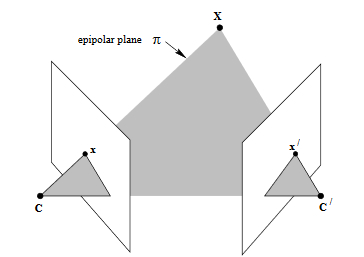
\includegraphics[width=12cm]{img/epipolar-1.png}
    \caption{Epipolar Plane Pictorially}
    \label{fig:epipolar}
\end{figure}

R, t are the relative transformation to get the second view from the first. Here, we have two cameras referring to a single point in the world coordinate system. But, imagine that we moved the point $X$ along the line described by $Cx$. The second camera would still capture the image. This essentially means that the possible world coordinates for a feature aren't unique! Looking closer at the image above, we can see that as we move $X$, we are tracing a line in the second image (with camera center $C'$). This is the epipolar line! Note that the epipolar line is a line on the image and hence a plane in euclidian space.

\textbf{Two Lines make a plane}

Intersection of the epipolar plane $\pi$ with the image plane (of the second camera) will give us the epipolar line. How do we form the epipolar plane? We need just 2 3D points to form a plane (take their cross product). We know cx already and cc' because the camera center has been transformed.

Let the epipolar line (on image 2) be represented as $l'$. To find the "stereo correspondence" for the point corresponding to x is what we need not cover the entire image plane but rather just the epipolar line.

Note that for every point on an image, we have an entire epipolar line on the other image.

An epipole is the point of intersection of the line joining the two camera centers with the image plane. The epipole in one image logically corresponds to the same point in the other image. 

\section{Fundamental Matrix}

"The fundamental matrix is the algebraic representation of epipolar geometry." As mentioned earlier, there was a mapping between point and epipolar line. This mapping is what is represented by the fundamental matrix. By multiplying the matrix with the point, we get a corresponding point in the other image.

\begin{figure}[h]
    \centering
    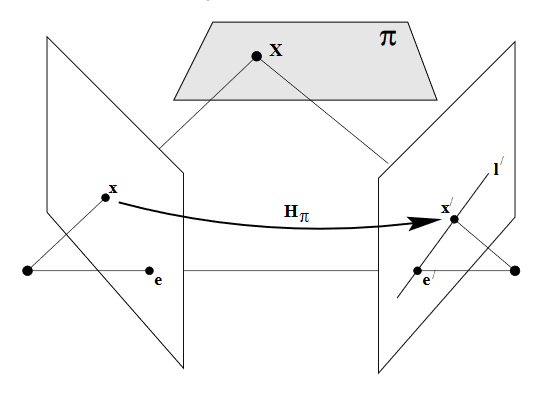
\includegraphics[width=12cm]{img/Fundamental_Matrix.png}
    \caption{A point $x$ in one image is transferred via the plane $\pi$ to a matching point $x'$ in the second image.}
    \label{fig:fundamental_image}
\end{figure}

\subsection{Geometric Derivation}

To derive F, we can look at it geometrically in two steps. From the book by Zisserman, the point $x$ is mapped to some point $x'$ in the other image lying on the epipolar line $l'$. This point $x'$ is a potential match for the point $x$. The second step, the epipolar line $l'$ is obtained as the line joining $x'$ to the epipole $e'$

Note that the points X, and x are projectively equivalent. Same for x'. Now, by projectivity theorem states that there exists a full-rank homography matrix $H_{\pi}$ such that:

There is a 2D homography from $x_i$ to $x_i'$.

\begin{equation}
    x' = H_{\pi}x
\end{equation}

Now, to get the epipolar line, we can take the cross product of two points which are on the line. If $e'$ is the point of intersection with the image with the line connecting camera centers, then the epipolar line is:

\begin{equation*}
    l' = e' \times x'=[e']_{\times} x' = [e']_{\times} H_{\pi}x = Fx
\end{equation*}

\textit{Note that above $[e']_{\times}$ is the skew symmetric matrix we use to find the cross product. Refer to the math section where we found that cross product operations can be written as a cross product.}

The fundamental matrix F may be written as $F = [e']_{\times}H_{\pi}$, where $H_{\pi}$ is the transfer mapping from one image to another via any plane $\pi$. This is a rank of matrix 2 - because $[e']_{\times}$ has rank 2 (only two degrees of freedom since it is a skew symmetric matrix).

Geometrically, we can imagine that F is a mapping from the projective plane to a particular epipolar line that passes through our epipole. Hence, it is a mapping from a 3 dimensional vector (2d projective space) to a 1 dimensional projective space. - from Zisserman 

Note: The plane need not exist! This can be imagined as two cameras at different heights at the same vertical angle can't form a plane. Given a point passing through a line, 

\begin{equation}
    x'^TFx = 0
\end{equation}

\subsection{Algebraic Derivation}

\begin{figure}[h]
    \centering
    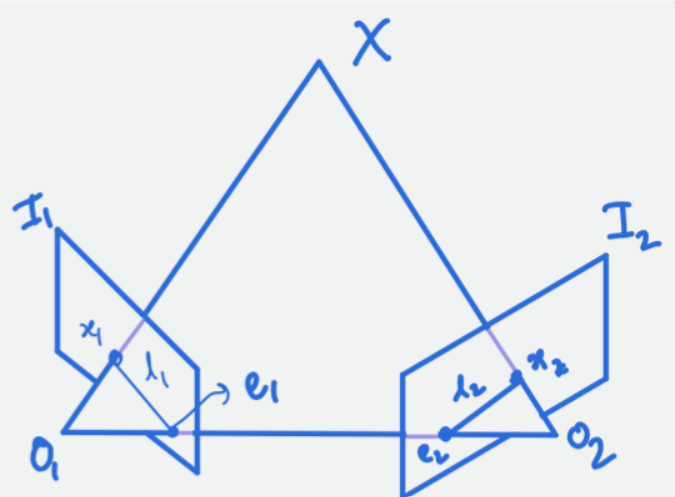
\includegraphics[width=12cm]{img/algebraic-fundamental.png}
    \caption{}
    \label{fig:Algebraic-fundamental}
\end{figure}

We will assume that the world coordinate system coincides with the camera coordinate system of our first image. Hence, we define:

\begin{equation*}
    O_1 = [I_{3\times3}|0_{3\times1}]
\end{equation*}

where this is the transformation between world coordinates to camera coordinates for frame 1. On the other hand, $O_2$ is the transformation to the second frame, which we will write relative to the first frame. That is, rotate and translate frame 1 to get frame 2. Hence,

\begin{equation*}
    O_2 = [R_{1\to 2}|t_{1\to 2}]
\end{equation*}

For simplicity, we will represent $R^2_1$ as rotation from 1st frame to 2nd frame.

Putting it all together, we have two set of equations:

\begin{equation}
\begin{split}
    &\lambda_1 \overrightarrow{p_1} = K[I|0]\overrightarrow{X}_{4\times1} \\
    &\lambda_1K^{-1}\overrightarrow{p_1} = \overrightarrow{X}
\end{split}
\end{equation}

Here, $K^{-1}\overrightarrow{p_1}$ is the normalized X coordinate $[X, Y, f]$ and $\lambda_1$ is the scaling factor. What is $\overrightarrow{p_1}$? This is the coordinate $[X, Y, 1]$ - the image coordinates.

The other equation is:

\begin{equation}
\begin{split}
    &O_2 = [R_{1}^2|t_{1}^2] \\
    &\lambda_2\overrightarrow{p_2} = K[R_1^2|t_1^2]\overrightarrow{X}\\ 
\end{split}
\end{equation}

Now, we know that $O_1O_2X$ forms the epipolar plane. Now, $O_1X$ is the same as $\lambda_1\overrightarrow{x_1}$. Now, we know that the dot product of two perpendicular lines is zero. Hence, we can write the following:

\begin{equation}
\begin{split}
    &\overrightarrow{O_1X}\cdot(\overrightarrow{O_1O_2} \times \overrightarrow{O_2X}) = 0 \\
    &\implies \lambda_1\overrightarrow{x_1}\cdot(\overrightarrow{t_1^2}\times R_2^1\lambda_2\overrightarrow{x_2}) = 0 \\
    &\implies \lambda_1\lambda_2\overrightarrow{x_1}(\overrightarrow{t_1^2}\times R_2^1\overrightarrow{x_2}) = 0\\
    &\implies \overrightarrow{x_1^T}[t_1^2]_{\times}R_2^1\overrightarrow{x_2} = 0 \\
    &\implies \overrightarrow{x_1^T}E_2^1\overrightarrow{x_2} = 0 \\
\end{split}
\end{equation}

Here, note that $\overrightarrow{O_1O_2}$ is represented by translation because that is in fact the transformation between the camera centers! Further, we are writing all these calculations in terms of frame 1. Hence, all coordinates have been transformed to the frame one relatives (by multiplying $R_2^1$ for instance). 

The matrix $E$ seen there is the \textbf{essential matrix} that relates points in terms of normalized pixel coordinates. E is the cross product of t and R, which also is in homogenous equation space, so translation gives 3 and rotation 3, but because of homogenization, we lose one degree of freedom. or $p^TEp=0$ and $p^T\lambda Ep=0$ which $\implies \lambda E = E$.

$F$ is something more - fundamental lol. 

\begin{equation}
\begin{split}
    &\implies  \overrightarrow{P_1}^TF_2^1\overrightarrow{P_2} = 0 \\
    &\text{ where $F_2^1 = K^{-T}[t_2^1]_{\times}R_2^1K^{-1}$}
\end{split}
\end{equation}

\subsection{Computation of $F$}

The fundamental matrix $F$ satisfies the equation $x'^TFx = 0$ and in order to calculate this matrix, we require at least 7 correspondence points (x maps to x'). 

* why there are 7 degrees of freedom *

I am lazy to write this part. Look at chapter 11 of the textbook for this section. 

\subsection{Normalized Eight Point Algorithm}



\subsection{RANSAC}

RANSAC isn't specific to multi-view geometry and can be used anywhere where there are outliers in our data. Now, with our data we will always have noise and we cannot choose any eight points and apply the eight point algorithm. RANSAC helps with this since outliers have little influence on the result. 

We will randomly take the minimum number of points required to determine the model parameters. Now, we can use the eight point algorithm and find the parameter. Then, determine how many points (from the set of all points) fit with the parameters chosen earlier. If the number of outliers are below a threshold, these parameters are acceptable. Repeat the same steps until the threshold has been met (if not met already obviously). 

The additional hyperparameters would be number of iterations, tolerance, etc. More about this can be read \href{http://www.cse.yorku.ca/~kosta/CompVis_Notes/ransac.pdf}{here}.

\section{Stereo Camera}

A stereo camera can be thought of as a special case of epipolar geometry - it is a combination of two monocular cameras separated by a fixed distance (lie on a common line called baseline). Now, if both cameras take an image and point to the same feature, we can find the world point.

Contrary to a monocular situation, with stereo cameras we know the exact distance between the cameras. 